\newpage

\chapter{Разработка системы моделирования.}
    \section{Разработка архитектуры приложения. }
    Разрабатываемая система позволяет пользователю строить  модель локальной сети, используя объекты, имитирующие поведение различного сетевого оборудования, проводить эксперименты в различных режимах работы, анализировать полученные результаты. Каждая из этих возможностей может быть реализована посредством подсистемы, которые являются компонентами проектируемой системы. Таким образом можно выделить следующие подсистемы.

    \begin{itemize}
        \item Подсистема моделирования. Данная подсистема отвечает за правильное взаимодействие компонентов модели, учитывая их параметры.
        \item Подсистема управления отвечает за сохранение(загрузку) параметров моделей, создание модели сети, а так же предоставляет методы для ее функционирования.
        \item Подсистема мониторинга отвечает за сбор данных в процессе моделирования и их анализ
    \end{itemize}

    \subsection{Подсистема моделирования. }

    Для реализации подсистемы моделирования необходимо описать взаимодействие различных компонент, входящих в ее состав. Такими компонентами являются модели устройств, протоколов, приложений. Объединение сетевых устройств реализовано в проектируемой системе посредством моделей сетевых соединений. Модель локальной сети представляет собой совокупность моделей устройств и их взаимодействия.

    \subsubsection{Канал связи. }

    Для имитации передачи данных могут быть использованы различные модели канала связи. При использовании модели идеального канала без помех единственной характеристикой такого соединения является задержка при передачи данных. В случае необходимости анализа передачи данных в каналах связи с помехами необходима реализация алгоритма генерации помехи. Используемая в системе модель канала связи представлена на рисунке~\ref{Pic2}.

    \begin{figure}[h!]\center
        \includegraphics[width = 60mm]{Ch3Pic2}
        \caption{Диаграмма классов модели канала связи. } \label{Pic2}
    \end{figure}

    Класс NoiseScript описывает алгоритм генерации помехи и связан с моделью канала связи через интерфейс Noise. Такая архитектура позволяет изменять использую модель канала связи без внесения изменений в архитектуру приложения.

    \subsubsection{Протоколы. }

    Для использования при моделировании различных сетевых протоколов они разбиты на четыре группы. К первой группе относятся протоколы, обрабатывающие данные приложений или вышестоящих протоколов. Каждый протокол, относящийся к этой группе, выполняет разделение данных на части и дополняет их служебными полями. В проектируемой модели, использующей стек протоколов TCP/IP, для каждого протокола эти фрагменты данных называются по-разному. Для Ethernet~--~кадры, для IP~--~пакеты, для TCP~--~сегменты. Структура взаимодействия протоколов отражена на рисунке~\ref{Pic3}.

    \begin{figure}[h!]\center
        \includegraphics[width = 40mm]{Ch3Pic3}
        \caption{Диаграмма классов модели протокола. } \label{Pic3}
    \end{figure}

    Анализ служебных полей фрагмента данных описывается в классе, реализующем интерфейс ProtocolScript. Данный механизм позволяет описывать различные протоколы для использования в системе, однако усложняет архитектуру приложения и описание процесса взаимодействия протокола.

    Второй группой протоколов, выделенных на этапе моделирования, являются протоколы управления средой. В стеке протоколов TCP/IP таким протоколом является протокол MAC-подуровня, уровня передачи данных. Отличительной особенностью этих протоколов является связь с устройством передачи данных и возможность контроля за передачей. На рисунке~\ref{Pic4} изображена диаграмма классов, используемая для описания этой группы протоколов.

    \begin{figure}[h!]\center
        \includegraphics[width = 100mm]{Ch3Pic4}
        \caption{Диаграмма классов модели протокола управления средой. } \label{Pic4}
    \end{figure}

    Интерфейс EnviromentControlProtocolScript предоставляет возможность описания различных протоколов управления средой. Для разрабатываемой модели будет реализован метод доступа с контролем несущей и обнаружением коллизий. Данный метод не используется в современных сетях с дуплексным каналом обмена информацией, однако необходим при использовании полудуплексного режима обмена данными.

    Алгоритм, описанный в классе EnviromentControlProtocolScript, определяет возможно ли начать передачу в данный момент времени, возможно ли считать передачу или прием данных успешными и, в некоторых случаях, определяет задержку передачи данных.

    Устройство передачи данных не выполняет никаких действий по контролю за процессом передачи данных, и является моделью передатчика, который генерирует необходимый сигнал и передает его в канал связи.

    Третьей группой протоколов являются служебные протоколы. В стеке протоколов TCP/IP таким протоколом является ARP. Он используется для установления соответствия между физическими адресами и адресами, используемыми на более высоком уровне модели. Для использования этого протокола необходимо внести изменения в архитектуру протоколов первой группы. Для этого добавляется еще один метод для отправки данных, использование которого сопряжено с запросом адреса, используемого на более низком уровне модели, соответствующего адресу на данном уровне. Взаимодействие протоколов первой группы и служебного протокола изображено на рисунке~\ref{Pic5}.

    \begin{figure}[h!]\center
        \includegraphics[width = 100mm]{Ch3Pic5}
        \caption{Схема взаимодействия протоколов передачи данных и служебного протокола. } \label{Pic5}
    \end{figure}

    Протоколы первой и третьей группы являются экземплярами одного и того же класса, который был расширен методами для операций по установлению соответствия адресов. Для подобного рода операций, служебные протоколы связаны с протоколами более низкого уровня, что позволяет им взаимодействовать независимо от адресов более высоких уровней модели.

    К четвертой группе протоколов относятся протоколы, связанные с приложениями. Данный вид протоколов предоставляет приложению интерфейс для обмена данными посредством локальной сети. В рамках используемой модели это протоколы четвертого уровня, содержащие в себе операции транспортного уровня, уровня представления данных и сеансового уровня. Учитывая сложность данных процессов, при реализации протокола TCP было принято решение выделить необходимые операции в отдельную подсистему. Диаграмма классов данной подсистемы представлена на рисунке~\ref{Pic6}.

    \begin{figure}[h!]\center
        \includegraphics[width = 100mm]{Ch3Pic6}
        \caption{Диаграмма классов транспортной подсистемы. } \label{Pic6}
    \end{figure}

    Интерфейс UserTransportFace предоставляет приложению методы для взаимодействия с транспортной подсистемой. Класс ConnectionControlSubsystem отвечает за установление, поддержание и закрытие TCP соединения. В этом классе определяются алгоритмы обработки данных в зависимости от состояния в котором находится соединение. Схема состояний и переходов представлена на рисунке~\ref{Pic7}. На данном уровне абстракции используется понятие сегмента данных. Начальное состояние системы - CLOSED. Управление соединением происходит посредством команд, поступающих от приложения и принятых служебных сегментов.



    \begin{figure}[h!]\center
        \includegraphics[width = 100mm]{Ch3Pic7}
        \caption{Схема конечного автомата TCP-соединения. } \label{Pic7}
    \end{figure}


    Типичный случай клиента, активно соединяющегося с сервером показан на жирными линиями - сплошными для клиента, прерывистыми для сервера. Тонкие линии обозначают необычные последовательности событий. Каждая линия маркирована парой событие/действие. Событие может представлять собой либо обращение пользователя к системной процедуре(CONNECT, LISTEN, SEND или CLOSE), либо прибытие сегмента(SYN, FIN, ACK, RST), либо, в одном случае, окончание периода ожидания, равного двойному времени жизни пакета. Действие может состоять в отправке управляющего сегмента(SYN, FIN или RST). Системные процедуры имеют следующее назначение:
    \begin{itemize}
        \item LISTEN - переводит систему в состояние ожидания соединений.
        \item CONNECT - попытка активного создания соединения.
        \item SEND - отправка данных.
        \item CLOSE - закрытие соединения.
    \end{itemize}

    Управляющие сегменты имеют следующее назначение:

    \begin{itemize}
        \item SYN - сегмент, отправляемый при установлении соединения.
        \item FIN - сегмент, отправляемый при закрытии соединения.
        \item RST - сегмент, отправляемый при сбросе соединения.
        \item ACK - сегмент, отправляемый для подтверждения получения определенного сегмента.
    \end{itemize}

    Назначение того или иного сегмента определяется наличием или отсутствием того или иного флага в TCP-заголовке сегмента.

    Класс SegmentControlSubSystem отвечает за гарантированную доставку сообщений. Это достигается за счет отправки сегмента данных до тех пор, пока не будет получено подтверждение об успешном его приеме.

    \subsubsection{Модели приложений.}

    Приложения, использованные в системе для моделирования действий пользователя, могут использовать протоколы разных уровней. Алгоритмы маршрутизации, используемые в коммутаторах работают на уровне передачи данных, а используемые в маршрутизаторах -- на сетевом уровне, как и алгоритмы генерации трафика. Модели уязвимостей используют транспортную подсистему.

    Приложение, используемое в коммутаторе, представляет собой алгоритм определения соединения, через которое будет направлен полученный пакет. Данный алгоритм имеет два режима работы. Первый - это режим обучения. В этом режиме составляется таблица соответствия физического адреса и порта коммутатора, к которому подключен абонент. При этом полученный пакет передается через все активные порты. Второй режим работы использует построенную на первом этапе таблицу маршрутизации для передачи пакета только указанному получателю. Исключением является широковещательный трафик.

    Построение моделей больших сетей требует использование маршрутизаторов для объединения рабочих станций в подсети и передачи трафика между ними. Приложение, описывающее процесс обработки пакетов, связано с протоколом сетевого уровня используемой модели взаимодействия и является упрощенной реализацией алгоритма маршрутизации. Для определения кратчайшего маршрута при передаче пакета, маршрутизатору необходима информация о состоянии сети и времени передачи пакета тем или иным путем. Для этого используются пакеты состояния линий. Каждый такой пакет содержит информацию об отправителе и "стоимости" пути под ближайших соседей. Для передачи этой информации всем маршрутизаторам в системе  используется алгоритм заливки. Он заключается в том, что каждый маршрутизатор передает полученный пакет на все выходы кроме того, по которому он пришел. Для предотвращения появления в сети большого количества повторных пакетов используется счетчик количества передач, по истечении которого пакет удаляется. Каждый пакет состояния, для определения его актуальности содержит свой порядковый номер. Получая такой пакет, маршрутизатор сверяется с имеющейся у него записью, и если полученный пакет обладает большим порядковым номером, то запись обновляется и пакет пересылается дальше. Если порядковый номер ниже, то пакет отбрасывается. Для сведения к минимуму фактов неверной отбраковки в случае сбоя в счетчике отправителя или ошибки в канале связи, каждый пакет содержит поле "Возраст". Данное поле записывается маршрутизатором и уменьшается на 1 каждую секунду. По истечении счетчика запись удаляется. Имея информацию обо всех маршрутизаторах в сети, для поиска кратчайшего маршрута используется алгоритм Дейкстры.[5]

    Генератор трафика = это приложение, предназначенное для имитации действий пользователя в системе, которые порождают сетевой трафик. На этапе построения моделей, для генераторов трафика было описано хаотическое отображение, описывающее состояние системы. На каждом интервале времени, для системы рассчитывается новое состояние, исходя из которого генерируется соответствующее количество трафика.

    Для моделирования процесса атаки на рабочую станцию, связанного с наличием уязвимости в приложении используем описанную модель активов и уязвимостей. Уязвимость отличается от актива только тем, что в случае удачной атаки, система считается скомпрометированной в то время, как удачная атака на один из активов подразумевает только получение некоторой информации. Для атаки на приложение злоумышленнику необходимо установить TCP-соединение с целевой рабочей станцией и послать соответствующий запрос. Приложение обрабатывает запрос и, с учетом параметров, влияющих на вероятность успеха, либо возвращает некоторую информацию, либо пустое значение, что означает, что атака была неудачной. Диаграмма классов, описывающая взаимодействие моделей приложений и транспортной подсистемы показана на рисунке~\ref{Pic8}

    \begin{figure}[h!]\center
        \includegraphics[width = 100mm]{Ch3Pic8}
        \caption{Диаграмма классов модели пользовательского приложения. } \label{Pic8}
    \end{figure}

    Абстрактный класс Application отвечает за загрузку и передачу данных уязвимостям(Vulnerability) и активам(Asset). Для реализации некоторого приложения, алгоритм его действий необходимо реализовать в классе-наследнике класса Application. На приведенном рисунке таким классом является ListenPortApplication. Данный класс создает TCP-сокет и переводит его в режим ожидания входящего соединения. Подобное поведение наиболее удобно для демонстрации процесса атаки, однако возможна реализация и более сложных алгоритмов.

    Модель поведения злоумышленника так же описывается в классе-наследнике от Application. При этом необходимо описать процесс формирования данных, которые будут отправлены приложению-жертве. В эти данные входит так же и параметры атакующего, такие как мотивация и уровень знаний.

    Каждая модель уязвимости или актива содержит таблицу, в которой хранятся вероятности успеха атаки в зависимости от характеристик атакующего и таблицу необходимой для успешной атаки информации, которая должна содержаться в сообщении злоумышленника.

    Таким образом, диаграмма классов, описывающая структуру модели сетевого устройства может быть изображена следующим образом(рисунок~\ref{Pic9}). Представленное изображение является упрощенным представлением архитектуры модели используемой в приложении. На нем отсутствуют вспомогательные классы, выполняющие различные операции с данными, суть которых не влияет на процесс обработки информации в целом.

    \begin{figure}[pH]\center
        \includegraphics[width = 140mm]{Ch3Pic9}
        \caption{Диаграмма классов модели сетевого устройства. } \label{Pic9}
    \end{figure}

    \subsection{Подсистема управления}

    Подсистема управления обеспечивает создание модели, ее функционирование, и является посредником между моделью и пользовательским интерфейсом, а так же подсистемой моделирования. Создание модели может производится двумя путями. Первый заключается в создании модели с помощью пользовательского интерфейса. При этом, оперируя готовыми моделями устройств и их настройками, возможно создание сетей различных конфигураций. Параметры моделей устройств хранятся в файлах XML, данные в которых разделены по подгруппам. Каждый файл отвечает за объекты, относящиеся к одной группе моделей. Такими группами являются модели приложений, модели стека протоколов, модели устройств. Таким образом модель конечного устройства, которая будет использоваться при моделировании, собирается из разных компонент, за загрузку которых отвечают классы NetworkConfigurationLoader, ApplicationManager. Параметры сетевых устройств, такие как адреса, загружаются классом Network в процессе создания сети. Для связывания данных, хранящихся в XML-файлах и объектов в программе используется набор интерфейсов, который называется JAXB(Java Architecture for XML Binding).

    Класс NetworkConfiguration реализует связывание данных, хранящихся в XML--файле с объектами приложения. По этим данным происходит построение модели модели сети на уровне взаимодействия устройств. Кроме этого, в файле сохраняется информация об используемых в каждом устройстве протоколов и приложений, что позволяет создать модель, описывающую взаимодействие компонентов одного объекта.

    \subsection{Подсистема мониторинга}

    Подсистема мониторинга решает следующие задачи:

    \begin{itemize}
        \item сбор данных, касающихся эффективности работы устройства;
        \item организация и отображение накопленных данных в формате, удобном для дальнейшего анализа;
    \end{itemize}

    Сбор данных в системе реализован посредством системы мониторов. Для этого создается объект-монитор, который сохраняет ссылку на наблюдаемый объект, и с определенной периодичностью снимает необходимые показания. В случае необходимости подсистема сбора данных запрашивает собранные данные и сохраняет их или выводит в форме графиков и таблиц. Взаимодействие компонент подсистемы моделирования представлен на рисунке~\ref{Pic17}

     \begin{figure}[h!]\center
        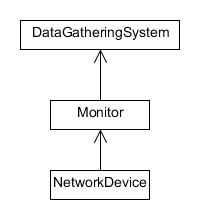
\includegraphics[width = 60mm]{Ch3Pic17}
        \caption{Схема взаимодействия компонент системы мониторинга. } \label{Pic17}
    \end{figure}

    Для оценки проблемы доступности данных, одним из наблюдаемых параметров является состояние очереди обработки пакетов сетевого устройства. Данный параметр непосредственно влияет на скорость реакции сервера, в случае поступления к нему запроса. Поэтому, для оценки этого параметра система моделирования позволяет вывести график, иллюстрирующий состояние очереди в каждый момент времени.

    Еще одной возможностью системы моделирования является проведение тестов на проникновение. Исход каждой попытки сохраняется в системе мониторинга отдельно для каждого устройства и при необходимости может быть проанализирован пользователем. Так же в эту таблицу для каждого устройства заносятся факты превышения определенной длины очереди обработки пакетов. Эта ситуация может свидетельствовать как о неправильной конфигурации устройства или неэффективной конфигурации сети, так и об атаке на отказ в обслуживании.



    \section{Описание работы приложения}

    \subsection{Создание модели}

    Для создания модели исследуемой сети предусмотрено несколько возможностей. Во-первых -- создание файла-конфигурации сети, с описанием всех устройств и соединений. При этом описание каждого устройства должно содержать список протоколов, которые используются устройством,  список приложений, с упоминанием используемых классов, описывающих действия приложения, уникальные идентификаторы устройства и адреса используемые в сетевом взаимодействии. Второй возможностью является использование пользовательского интерфейса. Данный интерфейс реализует механизмы, позволяющие пользователю создавать устройства с минимальными настройками, после чего проводить дополнительную конфигурацию в случае необходимости. Вид пользовательского интерфейса программы представлен на рисунке~\ref{Pic10}.

    \begin{figure}[h!]\center
        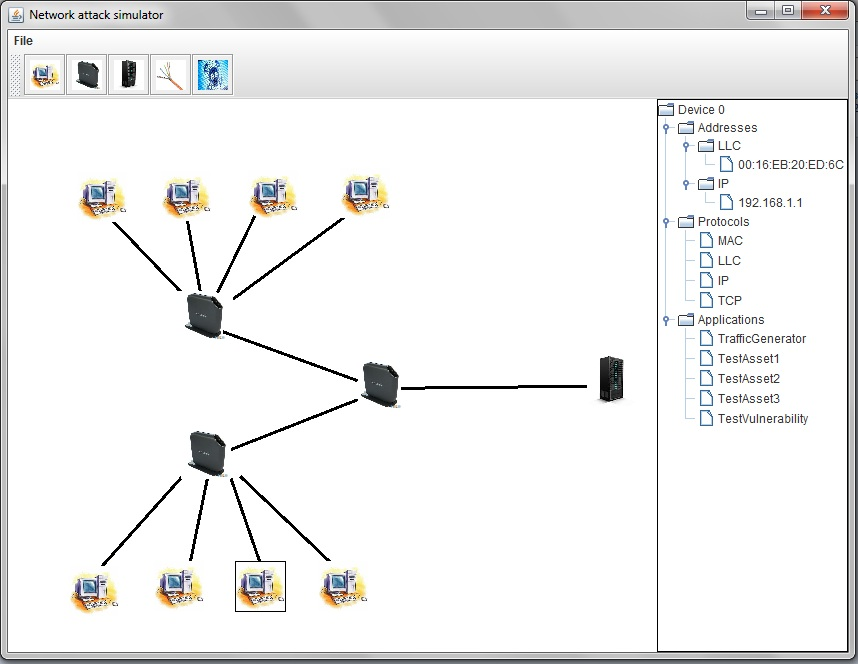
\includegraphics[width = 100mm]{SystemMainView}
        \caption{Диаграмма классов модели пользовательского приложения. } \label{Pic10}
    \end{figure}

    Главное меню приложения состоит из двух пунктов: File и Simulate. Меню File предоставляет функции по сохранению и загрузке различных моделей. Меню Simulate реализует возможности по управлению моделью и просмотру статистики по проведенным экспериментам.

    Панель, расположенная под главным меню, содержит кнопки для создания примитивов модели. Подсистема моделирования различает только два вида объектов - объекты-устройства и объекты-соединения. Различия устройств в характере обработки информации проявляются во внутренней конфигурации и используемых приложениях. Пользовательский интерфейс устанавливает дополнительные различия для удобства использования и, соответственно, задает устройствам различные начальные конфигурации. Объект "рабочая станция" представляет собой модель рабочей станции внутри локальной сети. Используемый стек протоколов - TCP/IP. В системе моделирования не рассматриваются различные виды трафика и протоколы, работающие выше транспортного уровня, поэтому единственным приложением, используемым по умолчанию является генератор трафика, который использует хаотическую функцию, описанную во второй главе. Объект "Сервер" отличается от объекта "рабочей станции" использованием в качестве приложения модели обработки входящего трафика и так же использует генератор трафика с иными параметрами хаотической функции. Каждое из описанных устройств имеет по одному сетевому порту. Объект "маршрутизатор" использует протоколы трех уровней модели взаимодействия: физического, передачи данных и сетевого, при этом с сетевым уровнем непосредственно взаимодействует алгоритм маршрутизации, реализованный как приложение низкого уровня. Маршрутизатор "по умолчанию" имеет 10 портов. Объект "Злоумышленник" по исходной конфигурации не отличается от рабочей станции и выделен в отдельную категорию для удобства управления его конфигурацией и поведением. Исходной конфигурацией объекта "соединение" является канал связи без помех.

    При выделении устройства открывается дерево его свойств, с помощью которого возможно изменить различные параметры устройства, добавить или удалить те или иные приложения и протоколы, однако, существует вероятность удаления необходимого для работы устройства компонента. В этом случае, некоторая часть модели может работать некорректно, что в свою очередь ведет к искажению результатов эксперимента.

    Для просмотра состояния какого либо из объектов предусмотрено использование контекстного меню, появляющегося при выделении устройства и щелчке правой кнопкой мыши. Это меню представлено на рисунке~\ref{Pic11}.

    \begin{figure}[h!]\center
        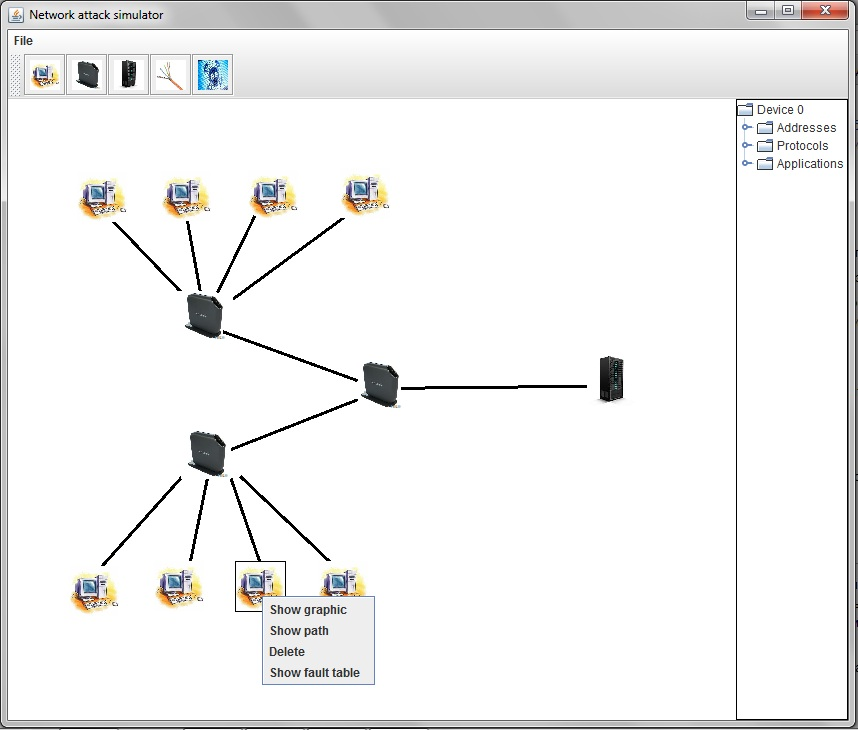
\includegraphics[width = 100mm]{contextMenuView}
        \caption{Диаграмма классов модели пользовательского приложения. } \label{Pic11}
    \end{figure}

    \subsection{Использование функций приложения}

    Для наглядности описания пользовательского интерфейса и возможностей программы, рассмотрим модель небольшой сети, состоящей из двух подсетей, объединяющих рабочие станции,  и сервера приложений. Исследуемой характеристикой в данном случае является состояние очереди обработки пакетов на сервере приложений, так как от нее зависит скорость, с которой пользователь может получить интересующие его данные. Для просмотра статистики по состоянию очереди необходимо вызвать пункт меню "Show graphic". Результат этой операции представлен на рисунке~\ref{Pic12}.

    \begin{figure}[h!]\center
        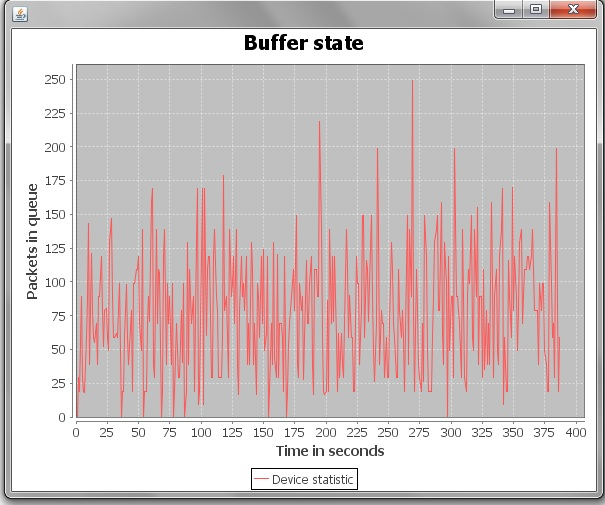
\includegraphics[width = 100mm]{LoadGraphic}
        \caption{График состояния очереди сервера. } \label{Pic12}
    \end{figure}

    На этом графике изображен размер очереди в различные моменты времени от начала моделирования. Для данного примера можно сделать вывод о том, что установка размера очереди в 1000 КБайт будет вполне достаточно для работы сети в нормальных условиях. Однако, манипуляции с интенсивностью трафика изменяют эту картину. Кроме количества пакетов в очереди, еще одной важной характеристикой является вид графика. На рисунке~\ref{Pic12} представлен график нормальной работы сервера, при
    которой он справляется с нагрузкой. Рассмотрим случай повышенной интенсивности трафика(рисунок~\ref{Pic13}).

    \begin{figure}[h!]\center
        \includegraphics[width = 100mm]{LoadGraphicOverload}
        \caption{График состояния очереди сервера. Перегрузка. } \label{Pic13}
    \end{figure}

    В данном случае график имеет вид неубывающей кривой, что сигнализирует о том, что сервер не справляется с генерируемой нагрузкой и в некоторый момент времени, независимо от максимального размера очереди возникнет перегрузка. В случае, если описанное поведение не является режимом DDos атаки, но является моделированием обычного режима, необходимо проверить параметры генераторов трафика устройств в сети и, если они адекватно описывают процесс генерации реального трафика в исследуемой сети, то необходимо пересмотреть конфигурацию сервера и, возможно, использовать более производительное оборудование.

    Еще одной возможностью программы является просмотр маршрутов трафика, связанного с некоторым объектом сети. Данная возможность включается в контекстом меню устройства, пункт "show path". При включении данной опции, каждое соединение, по которому проходит пакет с адресом получателя или отправителя эквивалентного адресу устройства, для которого задействована эта функция.

    На рисунке~\ref{Pic14} представлено использование этой функции для рассматриваемого примера. В данном случае, соединения, по которым проходит пакет с наблюдаемым адресом в поле отправитель окрашены в зеленый(\#00ff00) цвет, а поле получатель -- в голубой(\#00ffff). Эта опция позволяет отследить маршруты трафика для устройства и смоделировать возможности перехвата и перенаправления трафика.


    \begin{figure}[h!]\center
        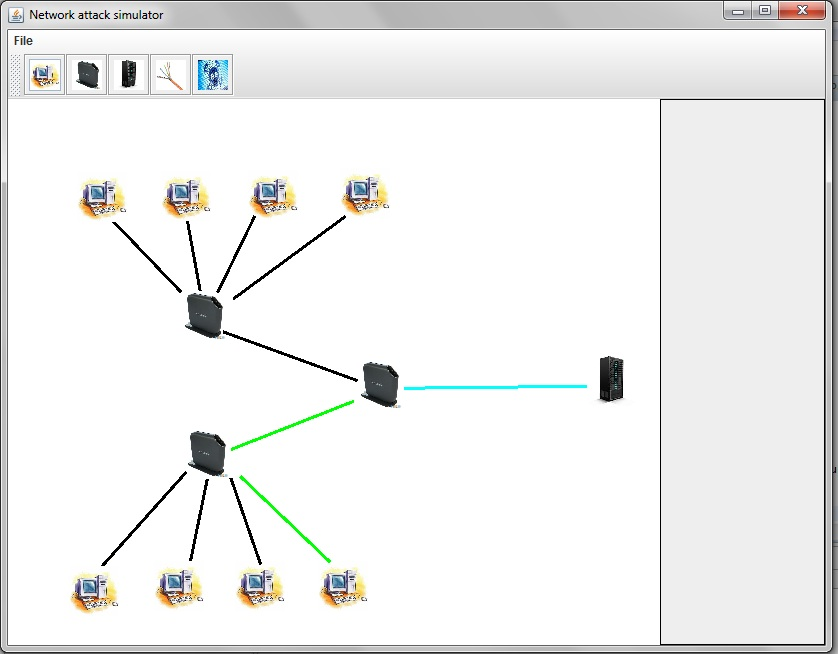
\includegraphics[width = 100mm]{routing}
        \caption{Маршруты пересылки пакетов для выбранного устройства. } \label{Pic14}
    \end{figure}

    Моделирование атак на проникновение не отображается на рассмотренном представлении модели и может быть проанализировано только посредством таблиц, в которых хранятся данные об атаках. Для этого используется пункт меню "show faults table". Faults table или таблица неисправностей представляет собой записи обо всех случаях, угрожающих нормальной работе устройства. Кроме рассматриваемых тестов в эту таблицу так же попадают записи о перегрузках в очереди устройства. В случае, если таблица неисправностей не пуста, устройство, которому она принадлежит приобретает рамку, окрашенную в красный цвет, которая отображается в независимости от того выделено устройство или нет(рисунок~\ref{Pic15}).


    \begin{figure}[h!]\center
        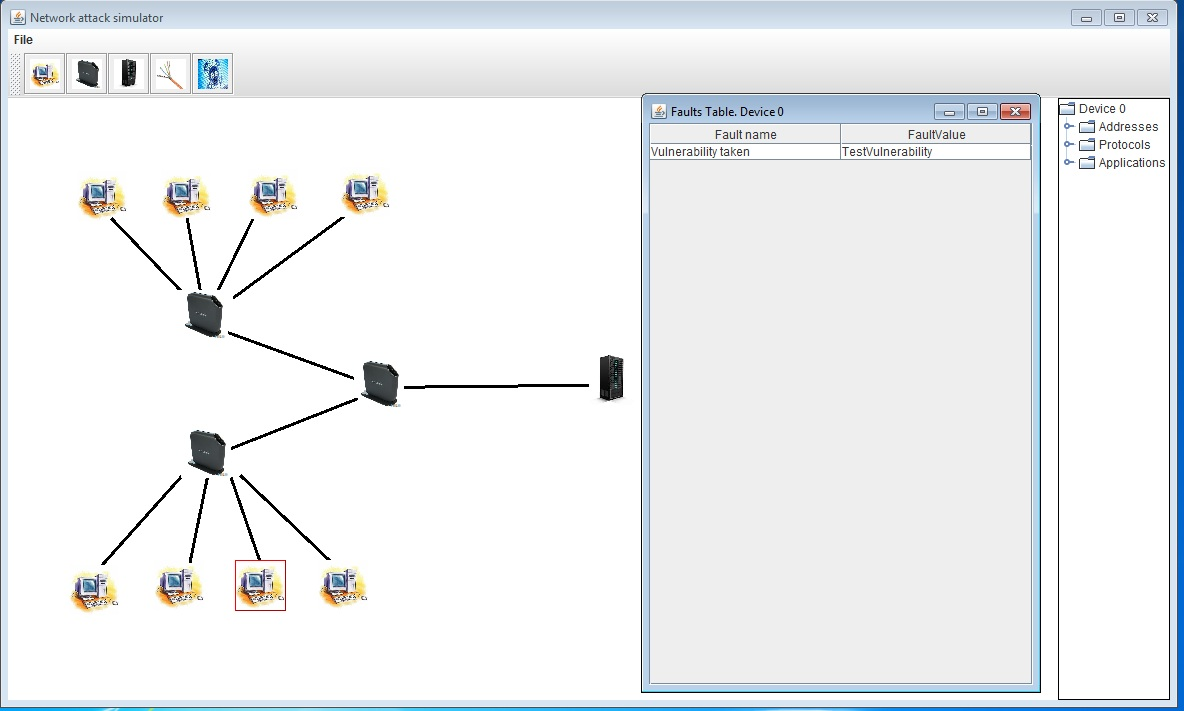
\includegraphics[width = 100mm]{FaultsTable}
        \caption{Таблица неисправностей для выбранного устройства. } \label{Pic15}
    \end{figure}

    Для рассматриваемого примера таблица неисправностей состоит из одной записи, что говорит о том, что имеющаяся в конфигурации устройства уязвимость была эксплуатирована злоумышленником. Однако по результатам одного теста нельзя говорить о степени защищенности той или иной сети или устройства в сети. Используемая модель проведения атак не гарантирует точного ответа на этот вопрос.

    Выводы о степени защищенности исследуемой системы можно сделать по результатам серии испытаний, для чего в меню "Simulate" выделен пункт "Statistics". На рисунке~\ref{Pic16} изображена такая таблица для семи испытаний. Эта таблица во многом повторяет значения таблицы неисправностей, но хранит эти значения для всех экспериментов, проведенных с моделью. По данным этой таблицы можно, при достаточном их количестве, можно провести статистическую оценку степени угрозы, которую представляет та или иная уязвимость.

    \begin{figure}[h!]\center
        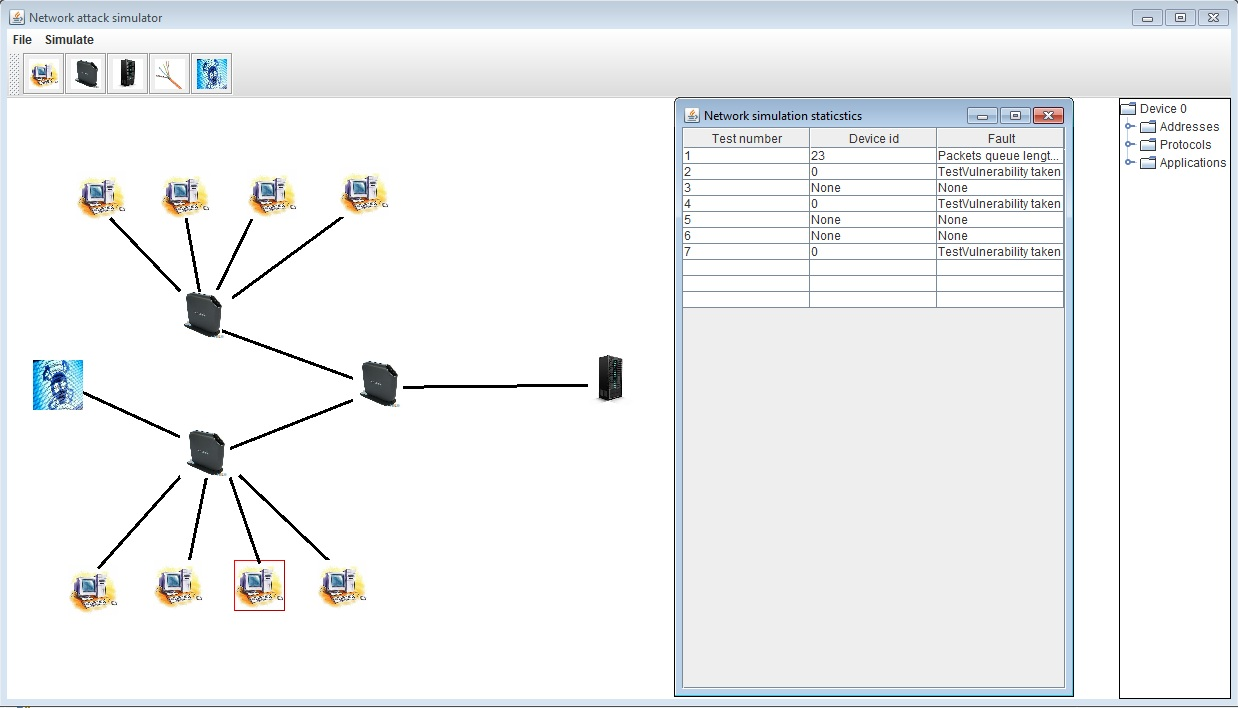
\includegraphics[width = 100mm]{StatisticsTable}
        \caption{Таблица результатов серии экспериментов. } \label{Pic16}
    \end{figure}

    \subsection{Анализ производительности}

    Рассмотренный пример является лишь способом описания возможностей системы и не является примером ее реального использования. Для сетей такого размера обычно не применяют методов моделирования, так как все неисправности, касающиеся производительности сети можно устранить в кратчайшие сроки. Методы имитационного моделирования используются в сетях с десятками и сотнями рабочих станций, организованных в подсети.

    Проведенный анализ показал возможность использования данной системы для моделирования средних и больших локальных сетей. Данные по анализу представлены в таблице~\ref{table1}
    \begin{table}[h!]
        \caption{Затраты вычислительных ресурсов ЭВМ при моделировании сетей различного размера}\label{table1}
        \begin{tabular}{|c|c|c|}

            \hline
            Количество устройств & Загрузка процессора & Используемая память(Мбайт) \\ \hline
            100 & 3\% & 260 \\ \hline
            200 & 5\% & 450 \\ \hline
            300 & 7\% & 610 \\ \hline

        \end{tabular}
    \end{table}

    Моделирование производилось на ЭВМ со следующими параметрами:

    \begin{itemize}
        \item Процессор Intel Pentium P6000 1.87GHz (2-ядра);
        \item Оперативная память 4Гб.
    \end{itemize}

    \subsection{Выводы}

    На данном этапе проектирования системы была реализована модель предметной области, описанная во второй главе, а так же другие компоненты системы моделирования, необходимые для проведения экспериментов. Реализованная модель предметной области представляет собой совокупность объектов, и процесса их взаимодействия. Каждый объект в свою очередь так же может быть разбит на несколько более мелких, реализующих те или иные его функции.

    Реализованная система позволяет проводить эксперименты, необходимы для оценки безопасности передачи данных в локальной сети, а также эффективность принимаемых мер по повышению защищенности. Несмотря на то, что некоторые возможности предоставляются пользователю готовыми к использованию, от него требуется наличие минимальных навыков по конфигурации сети, а так же знание о методах статистического анализа данных. При этом программа спроектирована таким образом, чтобы пользователь имел возможность внесения изменений в некоторые ее части, а именно, в файлы, описывающие алгоритмы поведения различных систем. В большей степени это касается алгоритмов приложений. Пользователь системы, обладая необходимыми навыками в программировании, может написать собственные модели приложений, отвечающие необходимым требованиям и более точно отражающие поведение используемых приложений и оборудования.

    Данная система может на ЭВМ различной мощности, так как не требует большого количества ресурсов, что показал проведенный анализ производительности. Однако моделирование больших вычислительных сетей может потребовать использования ЭВМ с большим объемом оперативной памяти. 